\documentclass[10pt
]{beamer}

\usepackage[english]{babel}
\usepackage[utf8]{inputenc}
%\usepackage[T1]{fontenc}
\usepackage{csquotes}
\usepackage[style=alphabetic,
citestyle=authoryear]{biblatex}
\usepackage{expex}
\addbibresource{biblio.bib}
\usepackage{booktabs}
%\usetheme[
%  workplace=phil,
%]{MU}
\usetheme{metropolis}
\AtBeginSection{
  \frame{
    \sectionpage
    \tableofcontents[currentsection]
  }
}
\usepackage{stmaryrd}
%\usepackage{natbib}
\usepackage{longtable}

\newcommand{\cond}[1]{\textsc{#1}}
\newcommand{\sem}[1]{\llbracket{#1}\rrbracket}


\title[Comparative and superlative differentials:\\
experimental evidence from Czech]{Comparative and superlative differentials:\\
experimental evidence from Czech}
\subtitle[SuB 26, University of Cologne]{Sinn und Bedeutung 26, University of Cologne}
\author[Mojmír Dočekal]{Mojmír Dočekal \& Hana Krajíčková}
\institute[FF MUNI]{Masaryk University}
\date{10-09-2021}
\subject{Presentation Subject}
\keywords{the, presentation, keywords}

\begin{document}

\begin{frame}[plain]
\maketitle
\end{frame}

\section{Basic Contrasts}
\begin{frame}{Modified Numerals}

\begin{enumerate}
    \item[i)] \alert{bare numerals}
    \pex
    This chocolate contains 25 grams of sugar.
    \xe

\end{enumerate}
\end{frame}

\begin{frame}{Modified Numerals}

ii) \alert{modified numerals}

\begin{enumerate}
    \item \alert{comparative modifiers (class A)} (\textit{more than, less than, over, ?no more than, ...})
    \pex
    This chocolate contains more than 25 grams of sugar.
    \xe
    \item \alert{superlative modifiers (class B)} (\textit{at most, at least, minimally, maximally, ...})
    \pex
    This chocolate contains at most 25 grams of sugar.
    \xe
\end{enumerate}

\footnotesize
extensive research: \cite{buring2008least,geurts2007least,nouwen2008upper,nouwen2010two,cummins2010comparative,kennedy2015fregean,alexandropoulou2016pragmatic}


\end{frame}


\begin{frame}{Modified Numerals and Existential Modals}

Comparative modifiers can scope under or over existential modals.


\pex This bus can carry fewer than 45 people.
  \a $\lozenge$ > \textit{fewer than 45} \hfill true - coach bus: 55 people
  \a \textit{fewer than 45} > $\lozenge$ \hfill true - city bus: 30 people
  \xe


\end{frame}

\begin{frame}{Modified Numerals and Existential Modals}

  Superlative modifiers have to outscope existential modals.

  \begin{itemize}
    \item the contrast crucial for our experiment
  \end{itemize}
  
  
   \pex This bus can carry at most 45 people.
    \a *$\lozenge$ > \textit{at most 45} \hfill false - coach bus: 55 people
    \a \textit{at most 45} > $\lozenge$ \hfill true - city bus: 30 people
    \xe
  
  \footnotesize
  
  \footnotesize
  \cite{geurts2007least,blok2019scope}
  
  
  \end{frame}
  

\begin{frame}{Ignorance Implicatures}
\begin{itemize}
    \item another important contrast
    \item sometimes related to the Maxim of Quantity: logically weaker sentences can signal speaker's ignorance
    \item comparative modifiers without ignorance implicature
\end{itemize}

\ex 
This chocolate contains more than 25 grams of sugar. \hfill no II
\xe

\begin{itemize}
    \item superlative modifiers with ignorance implicature

\ex This chocolate contains at most 25 grams of sugar. \hfill II
\xe 

\end{itemize}
\end{frame}


\section{Testing Czech \textit{no more than}}

\begin{frame}
  \frametitle{Testing Czech \textit{no more than}}

  \cite{nouwen2008upper} claims that \textit{no more than} is a comparative modifier since:

  \begin{itemize}
    \item both scopes in the existential modal env.
    \item no ignorance implicature (and with scalar bounding reading)
  \end{itemize}

\ex  Cody’s paper is allowed to have no more than 20 pages.  
\xe  

Both properties are intuitively inappropriate for Czech \textit{no more} ($\leftrightarrow$ motivation behind the experiments)

\end{frame}

\begin{frame}
  \frametitle{Differences between Czech and English \textit{no more}}

English \textit{no} can act as a determiner:

\pex \a No man arrived.
\a Every/the man arrived.
\xe

Unlike Czech \textit{no} in \textit{ne víc} which seems to be a focus particle

\ex \begingl
\gla \#Ne/$\checkmark$žádný muž nepřijel.//
\glb no/any man arrived//
\endgl
\xe

\end{frame}

\begin{frame}
  \frametitle{Differences between Czech and English \textit{no more}}

  Slavic focus particles (FP) have to (\cite{jasinskaja_information_2012} a.o.):
  
  \begin{itemize}
    \item c-command their associated F-marked expression
    \item be adjacent to the F-marked constituent
   
  \end{itemize}

\end{frame}

\begin{frame}

  Czech \textit{no} behaves like all other FPs, as exemplified in (\nextx) and (\ref{ex:seriously}) with a prototypical FP \emph{pouze} `only'
    

  \ex \hfill c-command
  \begingl
  \gla Já se choval {[}seriózně{]}\(_F\) *ne/pouze.//
  \glb I SE behaved seriously no/only.//
  \endgl
  \xe

  \pex\label{ex:seriously}\hfill adjacency
   \a I behave only {[}seriously{]}\(_F\). 
  \a I only behave {[}seriously{]}\(_F\). 
  \a
  \begingl
  \gla Já *pouze/*ne jsem se choval {[}seriózně{]}\(_F\).//
  \glb I *only/*no AUX SE behaved seriously//
  \endgl
  \a
  \begingl 
  \gla  Já jsem se choval pouze/ne {[}seriózně{]}\(_F\).//
  \glb I AUX SE behaved only/no seriously//
  \endgl
  \xe

\end{frame}

\begin{frame}

But the comparative morphology in Czech \textit{no more} is present: \textit{víc} is a comparative of \textit{mnoho} `much', \textit{než} `than' is used in the comparatives


\pex \a 
\begingl
\gla Petr měří ne víc než dva metry.//
\glb Petr measures no more than two meters//
\endgl
\a  
\begingl
\gla Petr je starší než Marie.//
\glb Petr AUX older than Marie//
\endgl
\xe

Summary of \textit{no more} vs. \textit{ne víc} diffs: 

\begin{itemize}
  \item both are built on a comparative base
  \item but \textit{no} is a determiner while \textit{ne} focus particle (constituent negation)
  
  \begin{itemize}
    \item being a focus particle, Czech \textit{no more} is close to focus sensitivity of \textit{at most/at least}: \cite{cohen2011superlative,coppock2013raising}
  \end{itemize}

\end{itemize}
 

\end{frame}

\begin{frame}
  \frametitle{Two Theories, Two Predictions}

\begin{enumerate}
  \item \cite{nouwen2008upper,nouwen2010two}: based on the morphology, \textit{no more than} -- comparative modifier
  \item \cite{kennedy2015fregean}: the difference between comparative and superlative modifiers comes from the ordering (semantics) -- strict (comparative) vs. non-strict (superlative)
  \begin{itemize}
    \item comparative \textit{fewer than 3}: $max < 3$ \hfill strict ord.
    \item superlative \textit{at most 3}: $max \leq 3$ \hfill non-strict ord.
    \item \textit{no more than}: can be treated as a superlative modifier (non-strict ord.)
  \end{itemize}
\end{enumerate}  
  

\end{frame}

\begin{frame}
  \frametitle{Predictions}

  \begin{longtable}[]{@{}llll@{}}
    \toprule
    & & $\lozenge >$\textit{no more than} & \textit{no more than} $> \lozenge$ \\
    \midrule
    \endhead
    Predictions & NMC as CM & \(\checkmark\) & \(\checkmark\) \\
    & NMC as SM & * & \(\checkmark\) \\
    \bottomrule
    \end{longtable}
  

\end{frame}

\begin{frame}
  \frametitle{Question Addressed by the Experiment}

  \ex If \textit{no more than} is SM, it should sound odd in a context preferring $\lozenge > $ \textit{no more than} interpretation.
  \xe

  \textbf{Question 1}

  \ex Does Czech \textit{no more} behave more like a comparative or superlative modifier (in the modal environment)?
  \xe


\end{frame}

\begin{frame}
  \frametitle{Question Addressed by the Experiment}


  \textbf{Question 2}
\ex Does Czech \textit{no more} behave like other differential quantifiers?
\xe

Consequences:

\begin{itemize}
  \item theoretical: support for one type of (modified) numerals theory;
  \item eventually distinguishing two types of differentials:
    \begin{enumerate}
      \item regular: \textit{slightly less}, e.g. (tested in the experiment)
      \item morphologically comparative but semantically superlative (Czech \textit{no more than})
    \end{enumerate}  
\end{itemize}

  

\end{frame}


\section{Experiment}

\begin{frame}
  \frametitle{Design}

\begin{itemize}
  \item joint work with Hana Krajíčková
  \item two experiments and two research questions:  
\end{itemize}
  
% \pex \a Does Czech \textit{no more} behave more like a comparative or superlative modifier (in the modal environment)? 
% \a Does Czech \textit{no more} behave like other differential quantifiers?
% \xe

Further: exp 2 -- included all the conditions of exp 1

\end{frame}

\begin{frame}
  \frametitle{Design}

  \begin{itemize}
    \item Czech native speakers 
    \item Likert scale 1-5
    \item  the appropriateness of one of the conditions in a context
    \item truth-value judgement task where a context described a situation strongly preferring the wide scope of the existential modal over the degree quantifiers
  \end{itemize}
\end{frame}

\begin{frame}
  \frametitle{Design}

\begin{itemize}
    \item 16 items and 16 fillers
    \item 98 subjects participated in the experiment (implemented on L-Rex), all of them passed fillers (uncontroversial TVJT)
    \item four conditions
  \end{itemize}
  

\end{frame}

\begin{frame}
  \frametitle{Design}

4 conditions:

\begin{enumerate}
  \item standard comparative modifier (\textit{méně než} `fewer than'): \cond{fewer}
  \item standard superlative modifier (\textit{nanejvýš} `at most'):  \cond{at-most}
  \item \textit{no more} modifier (\textit{ne víc než} `no more than'): \cond{no-more}
  \item standard differential comparative modifier (\textit{trochu méně než} `slightly less than'): \cond{slightly-less}
\end{enumerate}

\end{frame}

\begin{frame}
  \frametitle{Design}

  \begin{itemize}
    \item \cond{fewer} and \cond{at-most} tested the acceptability of modified numerals without differential
    \item \cond{slightly-less}, \cond{no-more} tested the presence of a differential (vague and zero degree differential)
  \end{itemize}
  
\end{frame}

\begin{frame}
  \frametitle{Design}

  The design was 2x2 factorial: 
  
  \begin{itemize}
    \item comparative vs. superlative modifier (\cond{classA},\cond{classB}) x 
    \item absence/presence of a differential (\cond{DiffYes},\cond{DiffNo})
    \item the main conditions:
    \begin{enumerate}
      \item \cond{fewer}: [+\cond{classA},-\cond{Diff}]
      \item \cond{at-most} [-\cond{classA},-\cond{Diff}]
      \item \cond{no-more} [-\cond{classA},+\cond{Diff}] \hfill contra \cite{nouwen2008upper}
      \item \cond{slighty-less} [+\cond{classA},+\cond{Diff}]
    \end{enumerate}
  \end{itemize}
  
\end{frame}

\begin{frame}
  \frametitle{Example item}

Context: Alex is reading the following sentence on a chocolate bar packaging:

  \pex[aboveexskip=0pt]   \begingl
  \gla Toto balení může obsahovat//
  \glb this packaging can contain//
  \endgl
  \a \hfill \cond{fewer}
  \begingl
  \gla méně než//
  \glb fewer than//
  \endgl
  \a \hfill \cond{at-most}
  \begingl
  \gla nanejvýš// 
  \glb at-most//
  \endgl
  \xe
  

\end{frame}

\begin{frame}
  \frametitle{Example item}

Context: Alex is reading the following sentence on a chocolate bar packaging:

  \pex[aboveexskip=0pt] 
  \begingl
  \gla Toto balení může obsahovat//
  \glb this packaging can contain//
  \endgl
  \a \hfill \cond{no more}
  \begingl
  \gla ne víc než//
  \glb no more than//
  \endgl
  \a \hfill \cond{slighty less}
  \begingl
  \gla trochu méně než  60 gramů cukru//
  \glb slightly less than 60 grams of-sugar//
  \endgl
  \xe

  Alex says: 'So, in this chocolate bar there can be sometimes even 65 grams of sugar.'

  

\end{frame}

\subsection{Results}

\begin{frame}
  \frametitle{Descriptive stats}

  \begin{itemize}
    \item the boxplot representing means and SEs below
  \end{itemize}


  

\end{frame}

\begin{frame}
  \frametitle{Boxplot}

\begin{figure}[htbp]
  \centering
  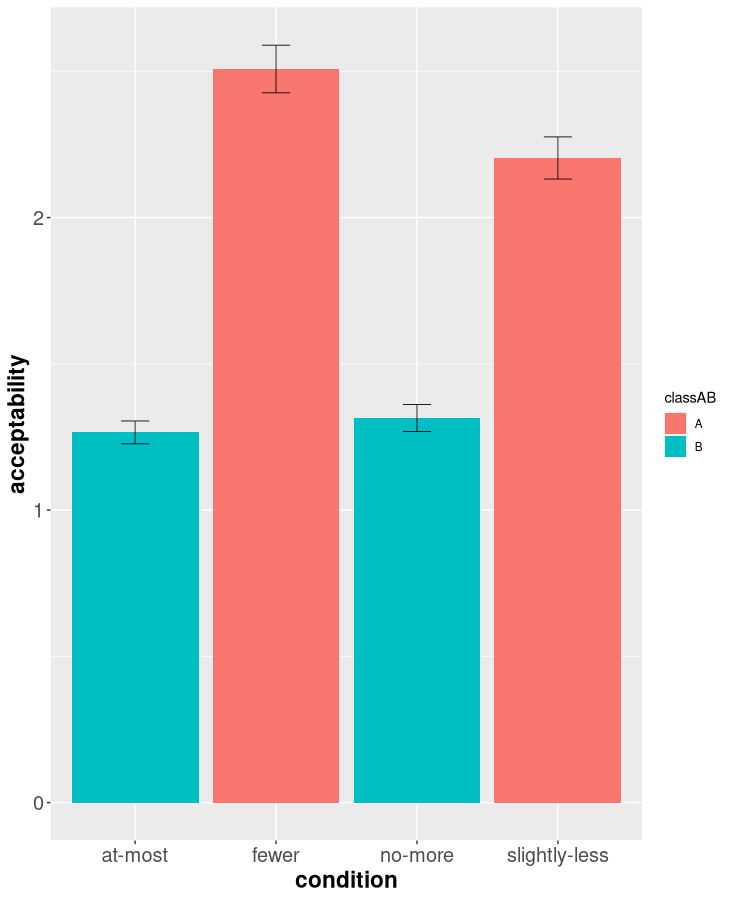
\includegraphics[scale=0.3]{plot_zoom_png.png}
  \caption{Boxplot of responses}
  \label{fig:boxplot}
\end{figure}
  

\end{frame}


\begin{frame}
  \frametitle{Results}

\begin{itemize}
  \item mixed-effects linear model with subject and item intercept+slope random effects (R package \textsc{lmerTest})
  \item dependent variable was the subject's response
  \item several models, and the one that describes data the best (the less fitting models included models with main effects only and models where \textit{no more} was treated as a CM):
  \item the model with independent variable conditions \cond{classA/B} vs. \cond{DiffYes/No} and their interaction
\end{itemize}

\end{frame}

\begin{frame}
  \frametitle{Results}

  \begin{itemize}
    \item negative main effect of \cond{classB} (SM) (t-value: -11.004, $p < 0.001$)
    \item positive effect of the absence of a differential (t-value: 3.946 $p < 0.001$)
    \item negative interaction of \textsc{classB} (SM) by \cond{DiffNo} (t-value: -3.129, $p =  0.002$)
    \begin{itemize}
      \item \cond{at-most} was less acceptable than \cond{fewer} considering that both of them are without differentials
    \end{itemize}
  \end{itemize}

\end{frame}

\begin{frame}
  \frametitle{Results}

  \begin{itemize}
    \item Tukey's pairwise comparison of the conditions: only \cond{at-most} and \cond{no-more} were statistically indistinguishable (t-value: -0.478, $p = 0.964$)
    \item all other pairs:  differed significantly
  \end{itemize}

\end{frame}


\begin{frame}
  \frametitle{Results}

The experiment confirms:

\begin{itemize}
  \item the scope behavior of Czech \textit{no more} construction follows the pattern of superlative, not comparative modifiers
  \item $\leftrightarrow$ subjects rejected \cond{no-more} to the same extent as \cond{at-least}
  \item the significant difference between \cond{no-more} and \cond{slightly-less}
  \item $\leftrightarrow$ \textit{no more} is a superlative differential quantifier and \textit{slightly less} as a comparative diff quant.
\end{itemize}

\end{frame}

\begin{frame}
  \frametitle{Results}

  Surprising result:
  
  \begin{itemize}
    \item low acceptability of all conditions: even the most default comparative modifier without a differential (cond \cond{fewer}) had $\mu$=2.51 (SD: 1.61, SE: 0.04)
    \item possibly priming effect of the most frequent everyday contexts like (\nextx), which strongly prefer the $max_d > \lozenge$ reading, just the opposite against the contexts described in our exp. 

  \end{itemize}

\ex 
\begingl
\gla Tato elektrokoloběžka může jet méně než 25 km/h.//
\glb this electric-scooter can run fewer than 25 km/h.//
\endgl
\xe

\end{frame}

\section{Analysis}


\begin{frame}
  \frametitle{Answers to the questions}

  \textbf{Question 1}

  \ex Does Czech \textit{no more} behave more like a comparative or superlative modifier?
  \xe

According to the scope behaviour in the existential modal env., it is a superlative modifier.


  \textbf{Question 2}
\ex Does Czech \textit{no more} behave like other differential quantifiers?
\xe


Czech \textit{no more} differs from the regular (comparative) differential (\textit{slightly less}).


  

\end{frame}


\begin{frame}
  \frametitle{Analysis}

  The scope behaviour of Czech NMC is of a superlative modifier profile
  
  \begin{itemize}
    \item generally: our exp confirms \cite{kennedy2015fregean}
    \item implementation:  there is no positive difference in degree between the arguments of the comparative \textit{more}
    
    \begin{enumerate}
      \item following \cite{nouwen2008upper}: analyze German/Dutch \textit{nicht mehr/niet meer} as a negative differential expressing  
      \item $\sem{\mathrm{nicht\ mehr\ }\alpha}=\lambda P.\neg \exists d'[max_d(P(d)) = \alpha + d']$ 
    \end{enumerate}

  \end{itemize}
  
\end{frame}

\begin{frame}
  \frametitle{Analysis}

  \begin{itemize}
    \item the negative differential analysis is equivalent to the superlative at-issue semantics of \textit{at most}
    \item in Kennedy's style of class A/class B analysis, we can classify Czech \textit{no more} as a superlative modifier
  \end{itemize}

  \pex \a $\lambda P.\neg \exists d'[max_d(P(d)) = \alpha + d']$
  \a $\approx \lambda P.max_d(P(d)) \leq \alpha$ \hfill (after \cite{kennedy2015fregean})
  \xe

\end{frame}

\begin{frame}
  \frametitle{Another approach}

  In \cite{zhang2021semantics} interval arithmetic decompositional approach

  \begin{itemize}
    \item both \textit{no more than 60} and \textit{at most 60} denote upper bounded closed interval:
  \end{itemize}
  
  \pex \a no more/at most than 60 \ldots $(-\infty, 60]$
  \a more then 60 \ldots $(-\infty, 60)$
  \xe

  Similar to the logic in \cite{kennedy2015fregean}: composition is semantically but not morphologically driven.


\end{frame}

\begin{frame}
  \frametitle{Analysis applied}


  The analysis correctly derives:
  
  \begin{enumerate}
    \item the wide scope of the class A modifiers \cond{no more} and \cond{at-most}:\\
    
    
    \ex $max_d(\lozenge \mathrm{contain}(\mathrm{ChocBar},d)) \leq 65g$
    \xe

    \item incompatible with Alex's continuation and predicts low acceptability of \cond{no-more} and \cond{at-most}
  \end{enumerate}

\end{frame}

\begin{frame}
  \frametitle{Analysis applied}

  The weak surface scope\\
  
  \ex $\lozenge[max_d(\mathrm{contain}(\mathrm{ChocBar},d)) \leq 65g]$
  \xe

  allowed only for comparative modifiers
  
\begin{itemize}
  \item explains the higher acceptability of \cond{fewer} and
  \cond{slightly-less} (whatever the reasons for obligatory wide scope of SM over existential modals are, see \cite{blok2019scope})
\end{itemize}
  
\end{frame}

\begin{frame}
  \frametitle{Consequences}

\begin{enumerate}
  \item morphology isn't always the right clue: Czech \textit{no more} behaves as a superlative modifier, despite its comparative morphology
  \item the experiment brings support for the CM vs. SM theory presented by \cite{kennedy2015fregean}: the distinction between class A/B = the type of ordering relation (strict vs. non-strict) -- \textbf{semantics}

  \begin{itemize}
    \item Czech \textit{no more} can be interpreted as $\neg$ (strict) $\rightarrow$ ordering entailments of non-strict ordering
    \item regular differential quantifiers (\cond{slightly-less}) remain strictly ordered, thus class A
  \end{itemize}

\end{enumerate}

\end{frame}

\begin{frame}
  \frametitle{Cross-linguistic speculations}

  So far: three types of NMC-languages: 
  
  \begin{enumerate}
    \item \textit{no more} as class A, English type of NMC (bounding inferences and both scopes w.r.t. existential modals)
    \item \textit{no more} as class B, Czech type of NMC (only $max_d > \lozenge$, lack of bounding inferences: \cite{docekal_upper_2017})
    \item languages where NMC depends on its realization behaves as CM or as SM (Hungarian according to Balázs Surányi (p.c.))
  \end{enumerate}
  
\end{frame}

\begin{frame}
  \frametitle{Cross-linguistic speculations}


  The variation seems to be related to  the morpho-syntactic status:
  
  \begin{enumerate}
    \item a focus particle/constituent negation in NMC (Czech) behaves as a superlative modifier
    \item a negative quantifier (English) in NMC leads to the comparative modifier behaviour
  \end{enumerate}

\end{frame}

\begin{frame}[plain]
\vfill
\centerline{Thank You for Your Attention!}
\vfill\vfill
\end{frame}

\section{\bibname}
\begin{frame}[t, allowframebreaks]{\bibname}
\printbibliography[heading=none]
\end{frame}


\end{document}

\title[Short Presentation Title]{Full Presentation Title}
\subtitle[Short Presentation Subtitle]{Full Presentation Subtitle}
\author[R. Speedwagon]{Robert Speedwagon\texorpdfstring{\\}{, }personal-id@mail.muni.cz}
\institute[FF MU]{Faculty of Arts, Masaryk University}
\date{\today}
\subject{Presentation Subject}
\keywords{the, presentation, keywords}
\begin{document}

\begin{frame}[plain]
\maketitle
\end{frame}

\section[Short Section 1 Name]{Full Section 1 Name}
\subsection[Short Subsection 1 Name]{Full Subsection 1 Name}

\begin{frame}{Frame Title}{Frame Subtitle}
plain text, \structure{page structure}, \alert{emphasis}
\begin{itemize}
  \item a single-line bullet list item
  \item a bullet list item that is quite long (in order to force a line break),
    which also contains \alert{emphasized text}
  \begin{itemize}
    \item a second-level list item
    \begin{itemize}
      \item a third-level list item
    \end{itemize}
    \item \alert{an emphasized second-level list item}
  \end{itemize}
\end{itemize}
\begin{enumerate}
  \item a numbered list item
  \begin{enumerate}
    \item a second-level list item containing a math expression
      \[ E = mc^2 \]
      and a citation \cite{einstein1905tragheit}
  \end{enumerate}
\end{enumerate}
\end{frame}

\subsection[Short Subsection 2 Name]{Full Subsection 2 Name}

\begin{frame}{Text Blocks}
text above a block\footnote{a footnote with an \url{https://address.edu}}
\begin{block}{Block}
  text in a block
\end{block}
\begin{exampleblock}{Example Block}
  text in a block
\end{exampleblock}
\begin{alertblock}{Emphasized Block}
  text in a block
\end{alertblock}
\end{frame}

\begin{frame}{Figures}
\begin{figure}
  \includegraphics[width=.5\textwidth,height=.5\textheight,keepaspectratio]{cow-black.mps}
  \caption{A standing Holstein Friesian cow%
    \footnote{%
      Will the cow ever lie down again?
      We may never know.
      \cite{tolkamp10cows}
    }%
  }
\end{figure}
\end{frame}

\subsection[Short Subsection 3 Name]{Full Subsection 3 Name}

\def\age(#1-#2-#3){%
  \the\numexpr(
    \year - #1
    \ifnum\month<#2
      - 1
    \else
      \ifnum\month=#2
        \ifnum\day<#3
          - 1
        \fi
      \fi
    \fi
  )%
}

\begin{frame}{Tables}
\begin{table}
  \begin{tabular}{llc}
    First Name & Surname & Age \\ \midrule
    Albert & Einstein & \age(1879-03-14) \\
    Marie & Curie & \age(1867-11-07) \\
    Thomas & Edison & \age(1847-02-11) \\
  \end{tabular}
  \caption{The great minds of the 19th century}
\end{table}
\end{frame}
